\documentclass[10pt,showpacs,preprintnumbers,amsmath,amssymb,nofootinbib,aps,prl,twocolumn,groupedaddress,superscriptaddress,showkeys]{revtex4-1}
\usepackage{graphicx}
\usepackage{dcolumn}
\usepackage{bm}
\usepackage[colorlinks=true,urlcolor=blue,citecolor=blue]{hyperref}
\usepackage{color}
\usepackage{listings}
\usepackage{subfig}
\usepackage{float}
\usepackage{tikz} % Send help 
\usepackage{physics}
\usepackage{algorithmic}


\lstset{ %
  basicstyle=\footnotesize,        % the size of the fonts that are used for the code
  breakatwhitespace=false,         % sets if automatic breaks should only happen at whitespace
  breaklines=true,                 % sets automatic line breaking
  captionpos=t,                    % sets the caption-position to bottom
  deletekeywords={...},            % if you want to delete keywords from the given language
  escapeinside={\%*}{*)},          % if you want to add LaTeX within your code
  extendedchars=true,              % lets you use non-ASCII characters; for 8-bits encodings only, does not work with UTF-8
  frame=single,                    % adds a frame around the code
  keepspaces=true,                 % keeps spaces in text, useful for keeping indentation of code (possibly needs columns=flexible)
 % language=Python,                 % the language of the code
  morekeywords={*,...},           % if you want to add more keywords to the set
  numbers=left,                    % where to put the line-numbers; possible values are (none, left, right)
  numbersep=5pt,                   % how far the line-numbers are from the code
  showspaces=false,                % show spaces everywhere adding particular underscores; it overrides 'showstringspaces'
  showstringspaces=false,          % underline spaces within strings only
  showtabs=false,                  % show tabs within strings adding particular underscores
  stepnumber=1,                    % the step between two line-numbers. If it's 1, each line will be numbered
  tabsize=2,                       % sets default tabsize to 2 spaces
}

\newcommand{\lexp}{\ket{\downarrow}}
\begin{document}
\title{FYS3150 Computational Physics - Project 4}
\author{Nicholas Karlsen}


\begin{abstract}
  Using the Metropolis algorithm to study a system of weakly coupled paramagnets, the Ising model. Derived exact solutions of expectation values for a 2x2 lattice and found that the required $\sim10^5$ Monte-Carlo cycles to consistent results with $\sigma\sim10^{-3}$.
\end{abstract}

\maketitle


\section{Introduction}
\section{Theory, Algorithms and Methods}
  \subsection{The Ising Model}
    In its simplest case, a paramagnet is described as a lattice of noninteracting dipole moments, each in a state up or down. Where the energy of the system is proportional to the sum of the spins, up or down of each noninteracting constituent.

    The Ising model is a natural extension to this, by adding local interaction between directly neighboring spins (See fig. \ref{fig:spinsites}), such that the energy of the system is instead proportional to the sum of the interactions of all coupled spins, which gives a more accurate description of the system compared to the simple case of an ideal paramagnet.

    Or more precisely, the energy is given by Eqn.~\ref{eqn:ising_energy}, where $s_i \in \{-1, 1\}$ and $J$ is a coupling constant.

    \begin{equation}
      E = -J\sum_{<kl>} s_ks_l
      \label{eqn:ising_energy}
    \end{equation}
    In this sum, the notation $<kl>$ means that we take the sum over each coupling $s_k s_l$.
    Consider again Fig.\ref{eqn:ising_energy}. The contribution, $\epsilon_i$, to the total energy due the interactions at spin-site $i$ is the sum of its interactions, $\epsilon_i = s_i(s_\uparrow + s_\downarrow + s_\leftarrow + s_\rightarrow)$ where the arrows denote the spin-site directly neighboring site $i$ in the direction of the arrow. Now wish to compute the energy contribution due to the interactions at the spin-site left of site $i$. In this case, the interaction between it, and spin-site $i$ has already been computed, and must not be counted again.

    \begin{figure}[H]
      \centering
      \begin{tikzpicture}
        [%%%%%%%%%%%%%%%%%%%%%%%%%%%%%%
        dot/.style={circle,draw=black, fill,inner sep=1pt},
        ]%%%%%%%%%%%%%%%%%%%%%%%%%%%%%% 
        \foreach \x in {-1,...,3}{
          \foreach \y in {-1,...,3}{
            % Draw 3x3 dot lattice
            \node[dot] at (\x,\y){};
            \node[dot] at (\x,\y){};
          }
        }
        \draw[thick, dashed] (1 + .1 , 1) -- (1 + 0.9, 1);
        \draw[thick, dashed] (1 - .1 , 1) -- (1 - 0.9, 1);
        \draw[thick, dashed] (1, 1 + .1) -- (1, 1 + 0.9);
        \draw[thick, dashed] (1, 1 - .1) -- (1, 1 - 0.9);
        % Text 
        \draw (1+.25, 1+.2) node{$s_{i}$};
      \end{tikzpicture}
      \caption{Section of a 2D lattice, where each spin-site is represented by a dot. In the Ising model, spin-site $i$ will only interact with its directly neighbouring spin-sites, connected by dotted lines in this diagram\label{fig:spinsites}}
    \end{figure}

    Further, in this project the lattice will be treated as pseudo-continuous where any spin-sites located at an edge, will also interact with the spin-site on the opposing edge, illustrated in Fig.~\ref{fig:ising_periodic bounds}, which strictly speaking constitutes having periodic boundary conditions. If instead we had fixed boundary conditions, there would simply be no such across-lattice interactions, and spin-sites located at the edges would then only interact with 3 other spin-sites (2 in the case of corner sites) in the 2D case.

    Much simpler, the net magnetization, $\mathcal M$, of the system is taken as the sum over all spins
    \begin{equation*}
      \mathcal M = \sum_i s_i
    \end{equation*}
      \begin{figure}[H]
      \centering
      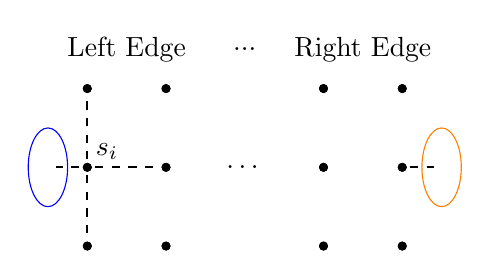
\begin{tikzpicture}
        [%%%%%%%%%%%%%%%%%%%%%%%%%%%%%%
        dot/.style={circle,draw=black, fill,inner sep=1pt},
        ]%%%%%%%%%%%%%%%%%%%%%%%%%%%%%% 
        \foreach \x in {2,...,1}{
          \foreach \y in {-1,...,1}{
            % Draw 3x3 dot lattice
            % LEFT LATTICE
            \node[dot] at (-\x,\y){};
            \node[dot] at (-\x,\y){};
            % RIGHT LATTICE
            \node[dot] at (\x,\y){};
            \node[dot] at (\x,\y){};
          }  
        }    
        % Lines
        \draw[thick, dashed] (-2, 0 + .1) -- (-2, 1 - .1);
        \draw[thick, dashed] (-2, 0 - .1) -- (-2, -1 + .1 );
        \draw[thick, dashed] (-2 + .1, 0) -- (-1 - .1, 0);

        \draw[color=blue] (-2.5,0) ellipse (0.25cm and .5cm);
        % Portal lines
        \draw[thick, dashed] (-2 - .1, 0) -- (-2.5 + .1, 0);
        \draw[thick, dashed] (2 + .1, 0) -- (2.5 - .1, 0);
        \draw[color=orange] (2.5,0) ellipse (0.25cm and .5cm);
        % Text
        \draw (0, 0) node{$\dots$};
        \draw (-1.5, 1.5) node{Left Edge};
        \draw (1.5, 1.5) node{Right Edge};
        \draw (0, 1.5) node{...};
        \draw (-2+.25, 0+.2) node{$s_{i}$};
      \end{tikzpicture}
      \caption{Spin-site $i$, located at the left edge of the lattice interacting with its direct neighbors, as well as the spin site on the opposite edge of the lattice
      \label{fig:ising_periodic bounds}}
    \end{figure}

    \subsubsection{Boltzmann Statistics}
      From this model we can derive many thermodynamic quantities by the use of Boltzmann statistics, where we have the probability of the system being in some specific macro-state\footnote{Macroscopic states being characterized by their energy, meaning i could just as well have written "... the probability of the system having some speciffic energy"} at temperature\footnote{Contained within $\beta$ in this notation}
      \begin{equation}
        \mathcal P(E_s) = \frac{1}{Z} e^{-\beta E_s}
      \end{equation}
      With $\beta \equiv \frac{1}{k_B T}$, the thermodynamic beta and $Z$, the partition function, acting as a normalization factor given by

      \begin{equation}
        Z = \sum_s e^{-\beta E_s}
      \end{equation}
      From this, the expectation value of some quantity $X$, with micro-states $X_s$ can be computed by

      \begin{equation}
        \left<X\right> = \sum_s X_s \mathcal P(E_s) = \frac{1}{Z} \sum_s X_s e^{-\beta E_s} 
        \label{eqn:expecval}
      \end{equation}
      Using this, we can compute the specific heat capacity, $C_V$ by computing the expectation values of $E, E^2$ \cite{statmek_lecnotes}, related by the following expression

      \begin{equation}
        C_V = \frac{\left<E^2\right> - \left<E\right>^2}{k_B T^2}
        \label{eqn:speciffic heat}
      \end{equation}
      Where $\left<X^2\right> - \left<X\right>^2$ is recognized as the variance of a set of randomly distributed quantities, $\sigma_X^2$.

      In a similar fashion, the magnetic susceptibility\footnote{Using the absolute magnetization to compute $\chi$, in line with the problem text for 4e}, $\chi$, is calculated from $\sigma_{\mathcal |M|} ^2$ \cite{statmek_lecnotes}

      \begin{equation}
        \chi = \frac{\sigma^2_\mathcal{|M|}}{k_B T}
        \label{eqn:suceptibility}
      \end{equation}

      For more details on the Ising model, or Boltzmann statistics refer to \textcite[Ch~6, 8.2]{schroeder}, \textcite{statmek_lecnotes}, or similar introductory texts on the topic.

  \subsubsection{Analytic solution of 2x2 Lattice}
    Consider now a 2x2 lattice, each with spin $\pm 1$.
    The energy of the system for a particular micro-state is given by Eqn.~\ref{eqn:ising_energy}, so for a $2\times2$ lattice we have

    \begin{equation}
      E = -J\sum_{<kl>}s_{kl} = -J\qty( 2s_1s_2 + 2s_1s_3 + 2s_2s_4 + 2s_3s_4)
    \end{equation}
    The multiplicity, that is number of possible combinations of micro-states for a system consisting of 4 spins is $2^4=16$.

     \begin{figure}[H]
      \centering
      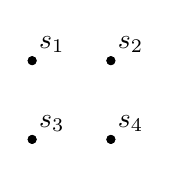
\begin{tikzpicture}
        [%%%%%%%%%%%%%%%%%%%%%%%%%%%%%%
        dot/.style={circle,draw=black, fill,inner sep=1pt},
        ]%%%%%%%%%%%%%%%%%%%%%%%%%%%%%% 
        \foreach \x in {0,...,1}{
          \foreach \y in {0,...,1}{
            % Draw 3x3 dot lattice
            \node[dot] at (\x,\y){};
            \node[dot] at (\x,\y){};
          }
        }
        \draw (0+.25, 1+.2) node{$s_{1}$};
        \draw (1+.25, 1+.2) node{$s_{2}$};
        \draw (0+.25, 0+.2) node{$s_{3}$};
        \draw (1+.25, 0+.2) node{$s_{4}$};

      \end{tikzpicture}
      \caption{A $2\times2$ lattice of spin-sites}
    \end{figure}

    If we first consider the micro-state in which all the spins are in parallel, we get energy $E=-8J$. Thus, this particular macro-state is at least 2-fold degenerate\footnote{Two micro-states corresponds to the same observable macrso-state.}.
    The different micro-states and their degeneracies are summed up in table \ref{tab:2x2energies} from \textcite{statmek_lecnotes}

    \begin{table}[H]
      \centering
      \caption{\label{tab:2x2energies} Possible configurations of 2x2 lattice}
      \begin{tabular}{llrr}
        No. spin up & Degeneracy & $E$ & $\mathcal M$ \\ \hline
        4 & 1 & -8J & 4 \\
        3 & 4 & 0 & 2 \\
        2 & 4 & 0 & 0 \\
        2 & 2 & 8J & 0 \\
        1 & 4 & 0 & -2 \\
        0 & 1 & -8J & -4 \\ \hline
      \end{tabular}
    \end{table}

    See that there are only 3 distinct energy macro-states, $E=-8J, 0, 8J$ corresponding to $2, 12$ and $2$ of the possible micro-states respectively.

    It is then easy to see that the partition function for the system will take the following form
    \begin{equation}
      Z = 2e^{+8J\beta} + 2e^{-8J\beta} + 12 = 4\cosh(8J\beta) + 12
    \end{equation}

    From this, we derive analytic values for $\langle E \rangle, \langle |\mathcal M| \rangle , C_V$ and $\chi$. 

    First, compute the expectation value of the energy using an alternate, simpler expression from \textcite[Ch~6.2]{schroeder}

    \begin{equation}
      \langle E \rangle = -\frac{1}{Z}\pderivative{\beta}Z = -\frac{8J\sinh(8J\beta)}{\cosh(8J\beta) + 3}
    \end{equation}
    Similarly, the expectation value of $E^2$ is computed easily by another expression found in \textcite[Ch~6.2]{schroeder}
    \begin{equation}
      \langle E^2 \rangle = -\frac{1}{Z}\frac{\partial^2}{\partial\beta^2}Z = - \frac{64J^2 \cosh(8J\beta)}{\cosh(8J\beta) + 3}
    \end{equation}
    From this, we compute the variance of $E$
    \begin{align}
      \begin{split}
        \sigma_E^2 &= \langle E^2 \rangle - \langle E \rangle ^2 
          \\
        &= \frac{-64J^2}{\cosh(8J\beta)+3} \qty(\cosh(8J\beta) + \frac{\sinh^2(8J \beta)}{\cosh(8J\beta) + 3})
      \end{split}
    \end{align}
    With which we can compute $C_V$ using Eqn.~\ref{eqn:speciffic heat}. Compute expectation values of $|\mathcal M|, |\mathcal M|^2$ using Eqn.~\ref{eqn:expecval} and Table~\ref{tab:2x2energies}

    \begin{align}
      \begin{split}
        \langle |\mathcal M | \rangle &= \frac{1}{Z} \sum_s |\mathcal M_s | e^{-\beta E_s} 
          \\
        &= \frac{8e^{8J\beta} + 16e^0}{Z} = \frac{2e^{8J\beta} + 4}{\cosh(8J\beta) + 3}
      \end{split}
    \end{align}

    \begin{align}
      \begin{split}
        \langle |\mathcal M |^2 \rangle &= \frac{1}{Z}\sum_s|\mathcal M_s|^2e^{-\beta E_s} 
          \\
        &= \frac{1}{Z}\qty(16e^{8J} + 32e^{0}) = \frac{4e^{8J\beta} + 8}{\cosh(8J\beta) + 3}
      \end{split}
    \end{align}
    We then compute the variance of the net magnetization
    \begin{align}
      \begin{split}
        \sigma_{\mathcal M}^2 &= \langle |\mathcal M|^2\rangle - \langle |\mathcal M|\rangle^2
          \\
        &= \frac{1}{\cosh(8J\beta) + 3}\qty(4e^{8J\beta} + 8 - \frac{4e^{16J\beta}+16}{\cosh(8J\beta) + 3})
      \end{split}
    \end{align}
    Which can be used to compute the magnetic susceptibility using Eqn~\ref{eqn:suceptibility}.
  \subsection{The Metropolis Algorithm}

\begin{lstlisting}[mathescape=true, language=python, title=Metropolis Algorithm]
Initialize State 

\end{lstlisting}

\section{Results and Discussions}

  See in Fig \ref{fig:convergence 2x2}

  \begin{figure*}[h!t]
    \center
    \subfloat[][$\langle E \rangle$]{
      \includegraphics[width=4.5cm]{figs/exb_convergencetest_E.pdf}
      }
    \subfloat[][$\langle |\mathcal M| \rangle$]{
      \includegraphics[width=4.5cm]{figs/exb_convergencetest_M_abs.pdf}
      }
    \subfloat[][$\langle C_v \rangle$]{
      \includegraphics[width=4.5cm]{figs/exb_convergencetest_Cv.pdf}
      }
    \subfloat[][$\langle \chi \rangle$]{
      \includegraphics[width=4.5cm]{figs/exb_convergencetest_chi.pdf}
      }
      \\
    \subfloat[][$\sigma_{\langle E \rangle}$]{
      \includegraphics[width=4.5cm]{figs/exb_convergencetest_E_std.pdf}
      }
    \subfloat[][$\sigma_{\langle |\mathcal M| \rangle}$]{
      \includegraphics[width=4.5cm]{figs/exb_convergencetest_M_abs_std.pdf}
      }
    \subfloat[][$\sigma_{\langle C_v \rangle}$]{
      \includegraphics[width=4.5cm]{figs/exb_convergencetest_Cv_std.pdf}
      }
    \subfloat[][$\sigma_{\langle \chi \rangle}$]{
      \includegraphics[width=4.5cm]{figs/exb_convergencetest_chi_std.pdf}
      }
    \caption{\label{fig:convergence 2x2} 
      (a-d) Computed results from running the algorithm 3000 times per number of monte-carlo cycles for 
      select expectation values with an ordered initial state of a 2x2 lattice of spin ups. (e-h) The standard deviation (Std.) of the computed results.
    }
  \end{figure*}



\section{Conclusions}

\bibliography{../bibliography.bib}


\end{document}  